\newpage
\section{Angles in a Funky Shape} 

\begin{teachingnote}
Nonconvex is better than concave.  Think of the amount of turning to identify which angle they are measuring.  Accuracy of protractor measurement.  Triangulation is the point of the angle sum.  An error worth discussing is triangulating incorrectly.
\end{teachingnote}
We are going to investigate the sum of the interior angles of a
funky shape.

\begin{prob}
Using a protractor, measure the interior angles of the crazy shape below:
\vspace{0.1in}
\[
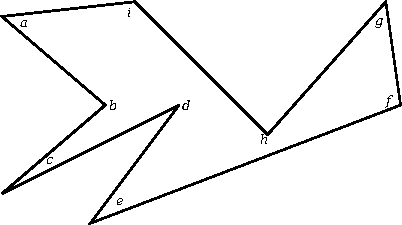
\includegraphics[scale=1.6]{../graphics/funkyshape.pdf}
\]
Use this table to record your findings:
\[
\vspace{0.1in}
{\renewcommand{\arraystretch}{1.5}
\begin{array}{|c|c|c|c|c|c|c|c|c|}\hline
a & b & c & d & e & f & g & h & i \\\hline
\rule[7mm]{10mm}{0mm}  & \rule[7mm]{10mm}{0mm}    & \rule[7mm]{10mm}{0mm}   & \rule[7mm]{10mm}{0mm}   &  \rule[7mm]{10mm}{0mm}   & \rule[7mm]{10mm}{0mm}    & \rule[7mm]{10mm}{0mm}   & \rule[7mm]{10mm}{0mm}   & \rule[7mm]{10mm}{0mm}   \\ \hline
\end{array}}
\]
\end{prob}

\begin{prob}
Find the sum of the interior angles of the polygon above. 
\end{prob}


\begin{prob}
What should the sum be? Explain your reasoning.  
(You might find it useful to consider some of the angles to be ``reflex angles.''  Which ones?)  
\end{prob}


